%% LyX 2.0.5.1 created this file.  For more info, see http://www.lyx.org/.
%% Do not edit unless you really know what you are doing.
\documentclass[english]{article}
\usepackage[T1]{fontenc}
\usepackage[latin9]{inputenc}
\usepackage{geometry}
\geometry{verbose,tmargin=2.5cm,bmargin=3cm,lmargin=2.5cm,rmargin=2.5cm}
\usepackage{amssymb}
\usepackage{graphicx}

\makeatletter

%%%%%%%%%%%%%%%%%%%%%%%%%%%%%% LyX specific LaTeX commands.
\newcommand{\noun}[1]{\textsc{#1}}
%% A simple dot to overcome graphicx limitations
\newcommand{\lyxdot}{.}


%%%%%%%%%%%%%%%%%%%%%%%%%%%%%% User specified LaTeX commands.
\usepackage{bbm}

\@ifundefined{showcaptionsetup}{}{%
 \PassOptionsToPackage{caption=false}{subfig}}
\usepackage{subfig}
\makeatother

\usepackage{babel}
\begin{document}

\title{Statistical Analysis of a Bike Sharing Transportation System}


\author{\noun{Juste Raimbault}$^{1,2}$\\
$^{1}$Erasmus Mundus Master in Complex Systems Science, Ecole Polytechnique
ParisTech\\
$^{2}$LVMT, Ecole Nationale des Ponts et Chauss�es}

\maketitle
\[
\begin{array}{ccc}
\star &  & \star\\
 & \star
\end{array}
\]


\bigskip{}
\bigskip{}
\bigskip{}


{\large \hfill{}}{\Large Erasmus Mundus Master in Complex Systems
Science}{\large \hfill{}\hfill{}}{\large \par}

\bigskip{}


{\large \hfill{}}{\Large Fall 2013 Project}{\large \hfill{}\hfill{}}{\large \par}

\bigskip{}
\bigskip{}
\bigskip{}


{\large \hfill{}}{\Large Class}{\large : }\textit{\large Therapeutic
Evaluation and Complex Systems}{\large \hfill{}\hfill{}}{\large \par}

\bigskip{}
\bigskip{}
\bigskip{}


\[
\begin{array}{ccc}
\star &  & \star\\
 & \star
\end{array}
\]


\bigskip{}
\bigskip{}



\section{Introduction}


\subsection{Context}

Bike Sharing system have recently been the object of common but also
scientific interest. The multiplication of implementation across many
countries of the world, following the example of European Cities,
has shown his potential as a new flexible and ecological transportation
system (\cite{demaio2009bike}). In \cite{midgley2009role} this new
transportation mode is presented as being totally complementary to
the overall transportation part of an urban system.\bigskip{}


It however raises particular issues in the conception and in the exploitation
of the system, because of the spatial and temporal heterogeneity in
use patterns. Therefore a consequent number of studies have been lead
in operationnal research in order to optimise the initial design of
the system (\cite{lin2011hub,lin2011strategic} for example) or the
bike redistribution process which is essential for maintaining a good
level of service (\cite{nair2011fleet,kek2006relocation}).\bigskip{}


The understanding of the mechanisms of such a system is essential
for a good management of it. Therefore one can use statistical models,
such as the work done on bike-sharing system of Lyon, for which statistical
cyclic models were used (\cite{borgnat2009studying,borgnat2009modelisation}),
including elaborated statistical estimators (\cite{michau2011peut})
and spatial analysis were done (\cite{borgnat2009spatial,jensen2010characterizing}).
An other approach is closer to datamining techniques, such as basic
visualisation of many systems (\cite{o2013mining}) or application
of clustering datamining techniques (\cite{vogel2011understanding,kaltenbrunner2010urban}).
We will place ourselves between the two approaches in the following.\bigskip{}



\subsection{Presentation of the project}

Our aim is to apprehend both generally and specifically a large set
of data representing exhaustively the working of a bike sharing system
during a given time period, that is Paris' bike-sharing system during
approximatively 3 months. That system, the largest in the world, has
been studied in \cite{nair2013large}. We want to extend this analysis
with other methods inspired from ones used on other systems. A part
of our work will be aimed at providing a statistical parametrisation
for an agent-based model that we won't detail here since that statistical
approach will have in itself self-consistence.\bigskip{}



\section{Data collection}


\paragraph{Type of data}

Data for the statistical analysis are public available data (open
data) from the bike-sharing system of Paris (``V'Lib''), provided
by the operating company in direct time on a dedicated website (url
\texttt{http://api.jcdecaux.com}, for which the format of request
is precised on \texttt{developer.jcdecaux.com}). It provides only
the status of docking stations at the request time so we had to automatize
the data collection process on a large time period in order to have
significant time-series. Process is detailed in the following.\bigskip{}


We chose to proceed that way for the data collection first because
the obtention of more precise data from the company can raise several
problems such as confidentiality issues or more constraining for our
research, lead to an lack of independence in the design of the modeling
process, since most of the time delivering of data had its price that
is at least answering to some question asked by the company. Secondly,
we argue that our experience will be one way of testing the possibilities
and limits of open data: if the public provided data can lead to relatively
good results compared to what can be obtained with a larger set. However,
if our research process becomes quickly limited by the lack of precision
or diversity in the data, that will bring one essential question on
front, that is that open data does not necessarly means freedom not
exhaustivity, and that the control of the provided data can implicitely
be highly dangerous for the global opening process. On that point,
we follow \noun{Banos} in \cite{banos2013HDR} when he argues that
a necessary condition of an open scientific cumulative process is
a total transparency in the methods and an exhausting sharing of implementations
of models of simulation and of data. Furthermore we wanted to avoid
any risk of implicit reporting spin since it stays a major issue today
for the quality of research as it is claimed by \noun{Ravaud} \& \textit{al}.
in \cite{boutron2010reporting}.

\bigskip{}


The purpose of data sharing by the company in our case was surely,
because of the nature of the available data, i. e. only current time
stations status, nothing more than current time information and mapping.
However, we will see that we can use them for statistical analysis
and obtain quite good results.\bigskip{}



\paragraph{Data collection process}

A script requesting current data to the API and saving it into a file
have been written and scheduled each 5 minutes on a remote server
(we did not choose finer temporal granularity for a material reason,
because the size of data becomes quickly huge and storage becomes
then an issue). Data on remote server is then zipped everyday for
storage purpose. When needed we download the files and process them
with R using \cite{couture2013rjson} in order to store them locally
on a reduced form (csv) that can be called directly by our data processing
algorithms. Note that it would have been more logical to process the
data remotely and store them under the reduced form but technical
reasons were an obstacle (in particular the installation of R on the
remote machine). We also extracted from extensive files static information
such as numerotation and coordinates of docking stations, what have
been useful after for example to create a geographical file for map
drawing with \cite{keitt2011rgdal}. Fig. 1 shows a flowchart of the
data collection and primary processing process. We collected data
for all Paris during around 3 month, following statistical analysis
are done on these data.

\begin{figure}


\hfill{}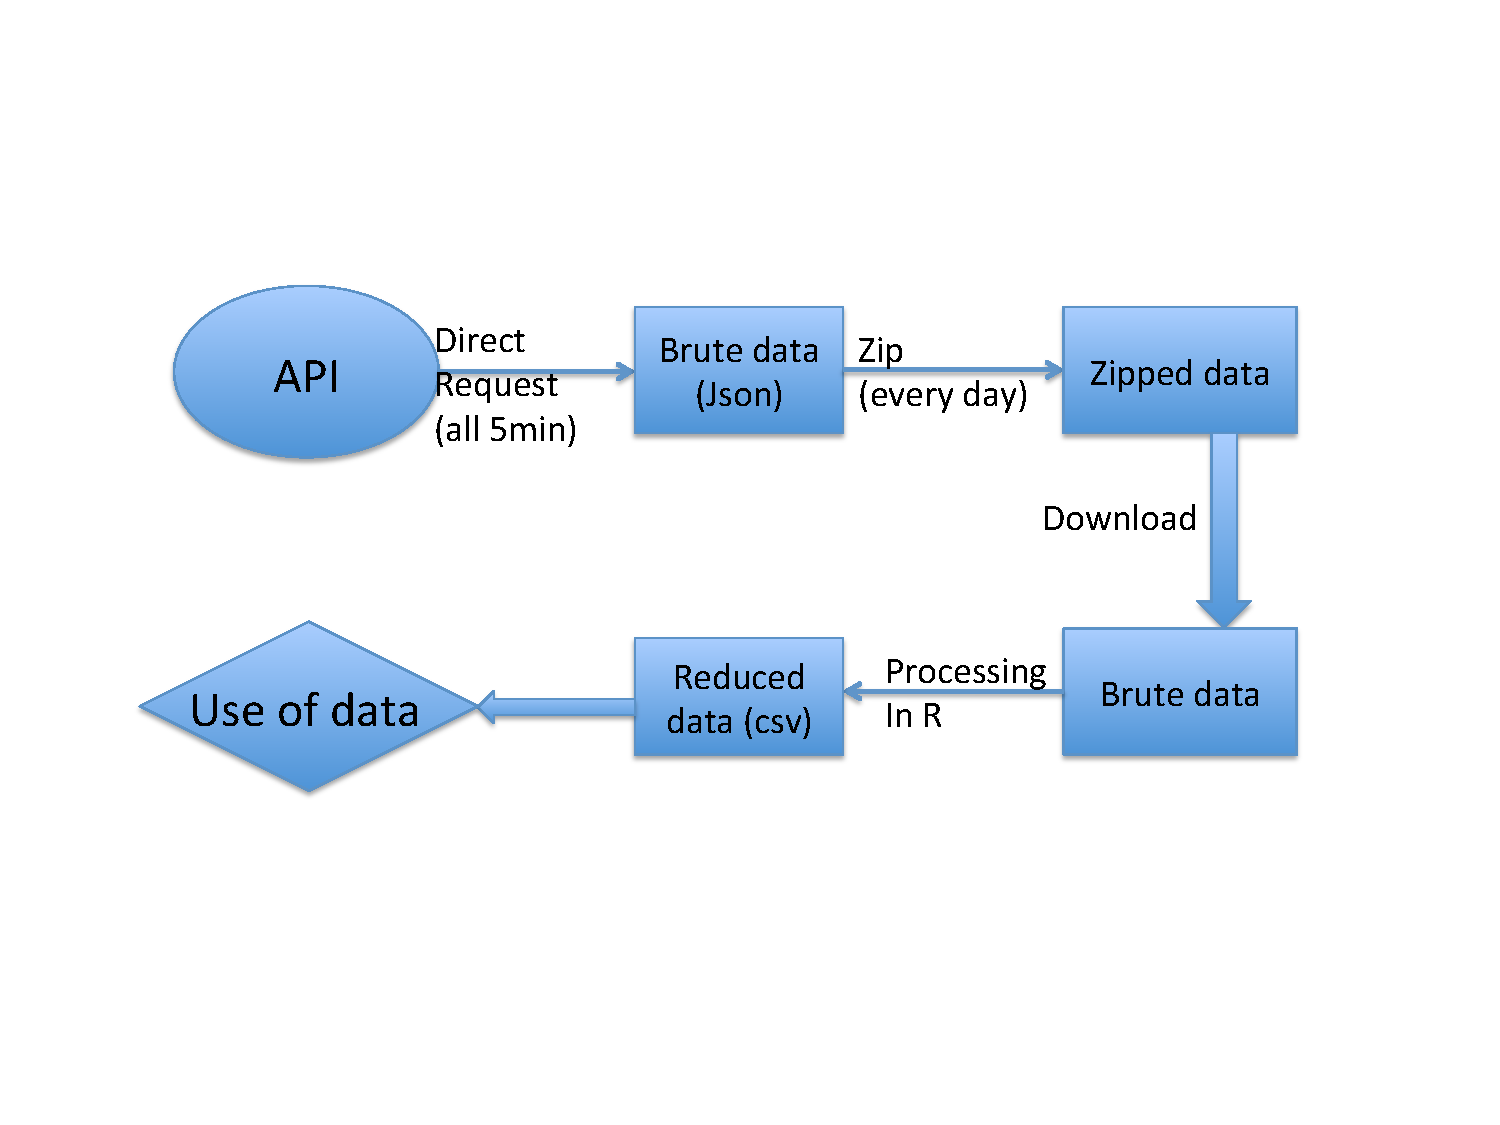
\includegraphics[bb=0bp 100bp 720bp 540bp,scale=0.45]{data}\hfill{}\hfill{}\caption{Flowchart of data collection process}


\end{figure}


\bigskip{}



\section{Statistical analysis}


\subsection{Data visualisation}

Many basic means for a global visualisation of data behavior are available
such as the ones proposed in \cite{o2013mining}, so we won't go too
much into detailed representation since it is not the first puspose
of our study. Note that this step is however essential, especially
during the elaboration of algorithm and the choice of methods for
statistical treatment.

\bigskip{}


To have an idea of the cyclic character of daily mobility patterns,
we can plot the total number of available bikes at docking stations
against time. If we suppose the total number of bikes constant over
the time duration of the plot, what seems reasonnable even on the
all time period our data cover (even if there are surely variations
because for example of bike reparations, they are surely neglectible
regarding the total number of bikes, which is around 15000), this
plot is exactly the complementary of the quantity of current travel
as a function of time, what allows to visualize mobility tendancies.
Fig. 2 shows the obtained curve that fits the expected results, showing
in particular the distinction between week days and weekends.

\begin{figure}
\hfill{}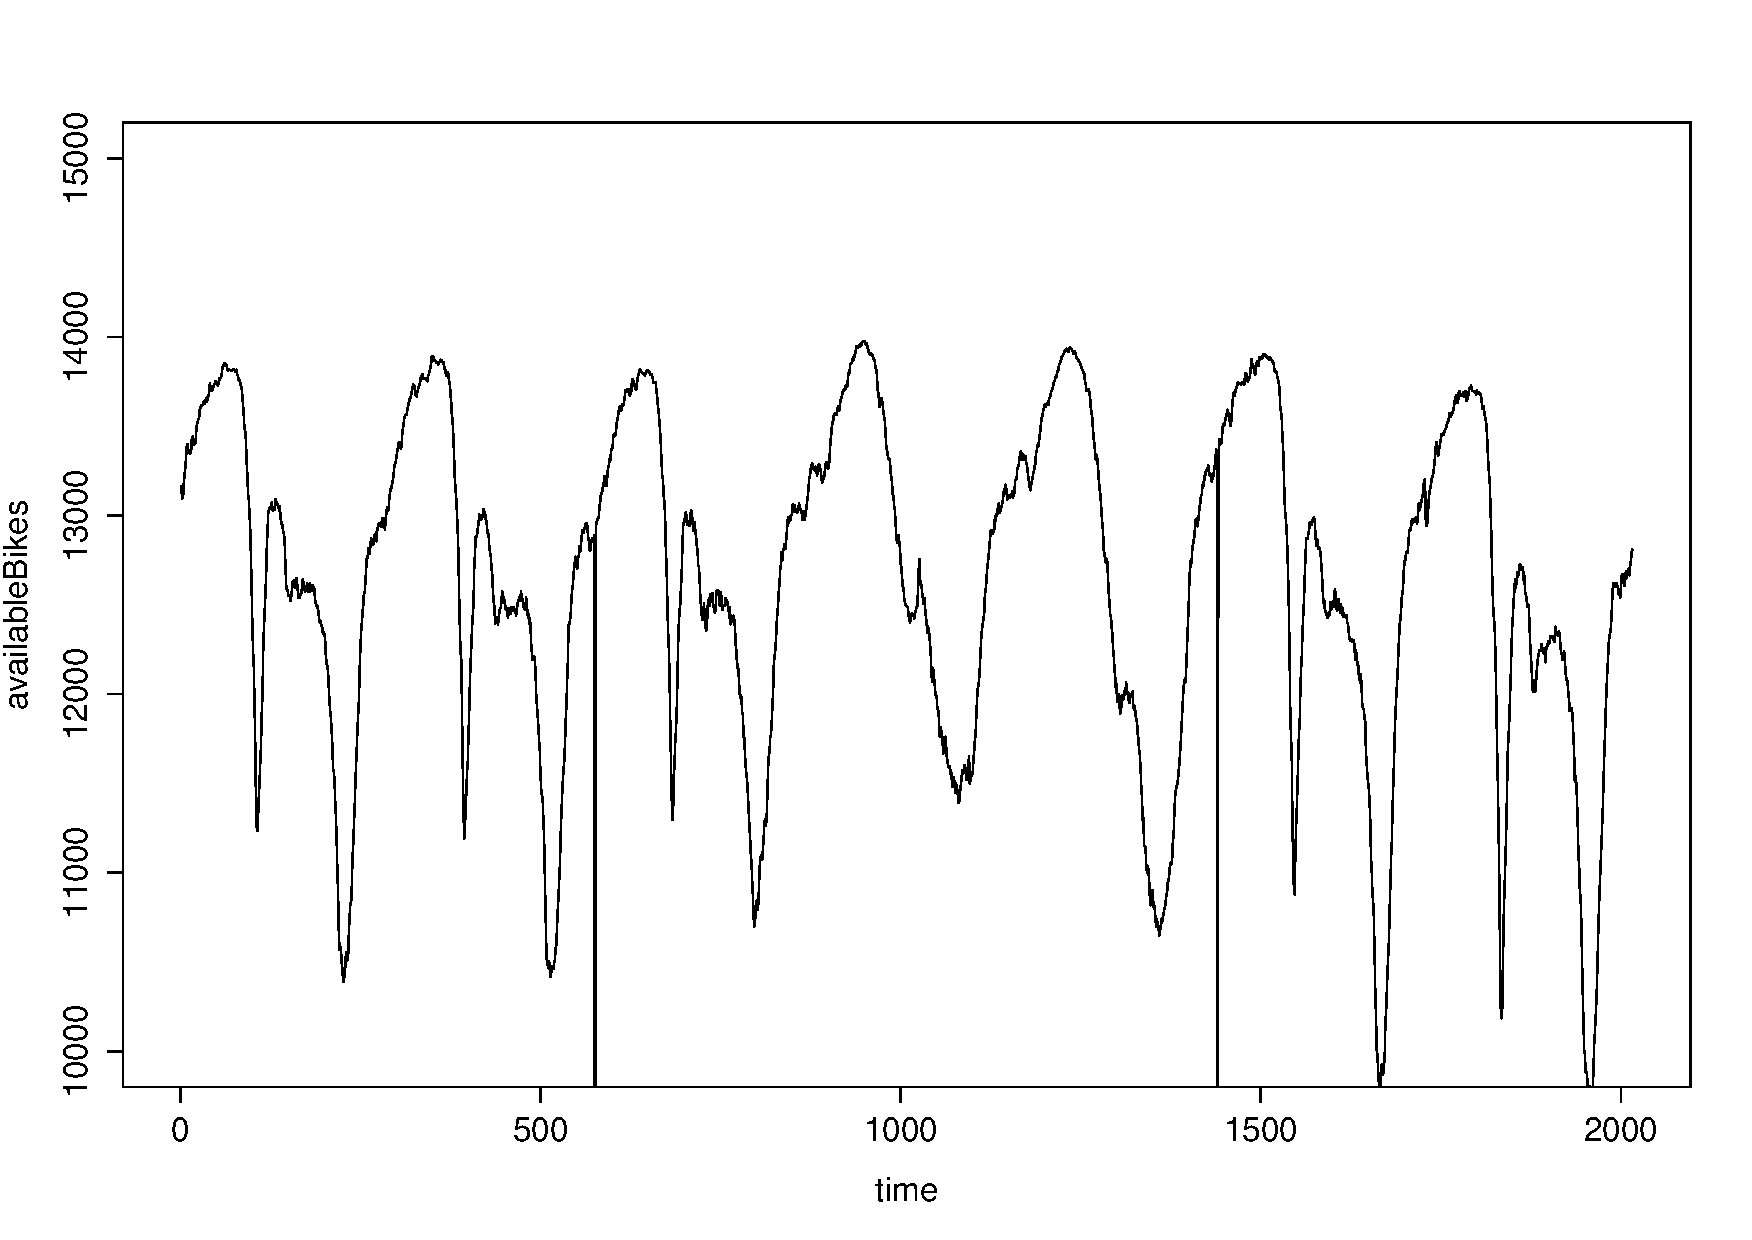
\includegraphics[scale=0.45]{/Users/Juste/Documents/ComplexSystems/CityBikes/Results/Visu/availableBikes}\hfill{}\hfill{}\caption{Quantity of total available bikes over a week. We observe the typical
patterns of the daily mobility, with two minima corresponding to morning
and evening affluence. The two day in the middle correspond to saturday
and sunday since the serie begins on a wednesday. These weekend days
present only one minimum, what is logical (no affluence in the morning)
and confirms the results of other studies.}


\end{figure}


\bigskip{}


We can also for example draw maps for the understanding of spatial
patterns in system use. One can expect for example to see distinction
in time between residential and activity areas for the quantity of
available bikes in stations. This allows to visualise global and local
heterogeneity patterns. Fig. 3 shows an example of such maps on a
particular district.

\begin{figure}
\subfloat[Midnight]{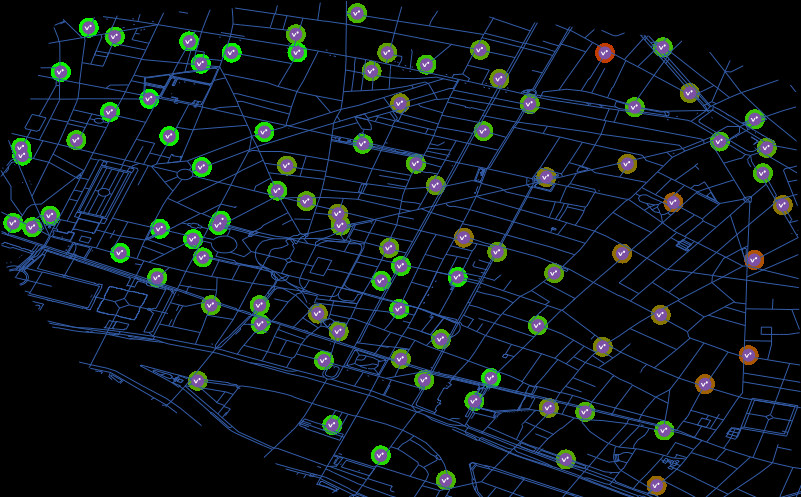
\includegraphics[scale=0.3]{/Users/Juste/Documents/ComplexSystems/CityBikes/Results/Views/lfmidnight}

}\subfloat[Midday]{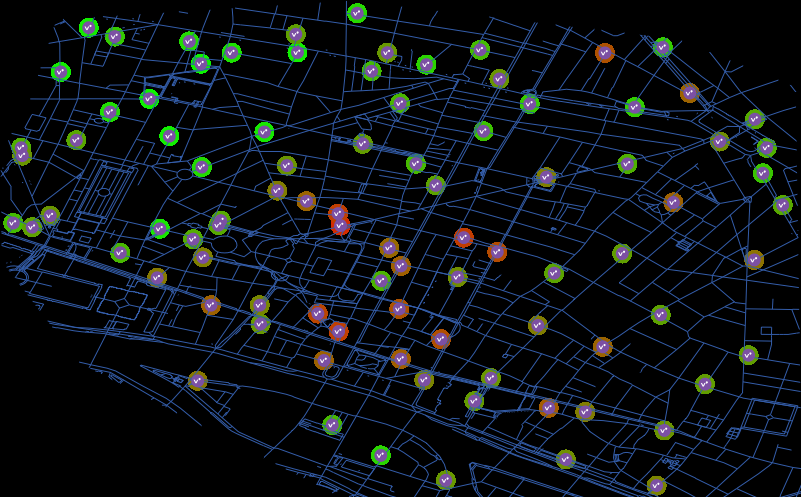
\includegraphics[scale=0.3]{/Users/Juste/Documents/ComplexSystems/CityBikes/Results/Views/lfMidday}}

\caption{Examples of heatmaps at two different moments of the day for the district
of Chatelet. The color indicates, from green that corresponds to an
empty station, to red to a full one, number of available bikes. Since
it is a working district and not residential, stations in the center
are overloaded during the day but empty during the night as expected.}
\end{figure}



\subsection{Extraction of patterns}

A first step in the treatment of data is to extract typical patterns
in use of the system. In \cite{vogel2011understanding}, datamining
techniques, and especially clustering of activity profiles, are used
to extract typical patterns in station use. We propose to use similar
methodology in order to identify typical overall day profiles and
classify them. We expect to be able to differentiate weekdays from
week-ends for example, but also see the influence of climate on use
patterns. The clustering of time-series offer an alternative for a
predictive model, as the cyclic model proposed in \cite{borgnat2009modelisation,borgnat2009studying}.\bigskip{}


A day is exhaustively represented by the time-series, defined on all
the stations of the system $s\in S$, and on a discrete time sample
$T=\{0,\tau,...,N\tau\}$ (with $\tau$ time step of the data, 5min
in our case), $(b(s,t))_{s\in S,t\in T}$ of availables bikes at each
stations. Each station has a maximal capacity $c(s)$ that allow to
define the number of free parking places $p(s)=c(s)-b(s)$ and the
load factor wich can be more convenient to work with since it is normalised
$lf(s)=\frac{b(s)}{c(s)}$. The overall clustering process first aims
to reduce the dimension of the representation of a day without loosing
majority of information, and then to be able then to classify days
and make predictions on the day characteristics from its data.

\bigskip{}


First the dimension is reduced through a sampling process that can
be seen as a projection from the space of complete time-series to
a space of smaller dimension. If $\varphi\in\mathbb{N}^{\mathbb{N}}$
is a extraction then the sampling is defined as the canonic projection
$\mathcal{S}:\mathbb{R}^{\left|T\right|\left|S\right|}\rightarrow\mathbb{R}^{\left|\varphi(T)\right|\left|S\right|}$.
The question of the value of the time step for sampling is important.
We tried for many values and looked at the possible loss of information
through the evolution of clustering coefficient regarding number of
clusters. It appeared that we had still good precision for large time
steps such as one hour. See fig. 4 for more precision on the influence
of sampling step.\bigskip{}


\begin{figure}
\hfill{}\subfloat[Clustering coefficient as a function of cluster number for different
values of sampling step. The more blue the curve is, the more sampling
step is large. If the curve goes quickier to 1, that means that points
are less distinct and that statistical distribution contains less
information. We observe a jump that is quantified in (b).]{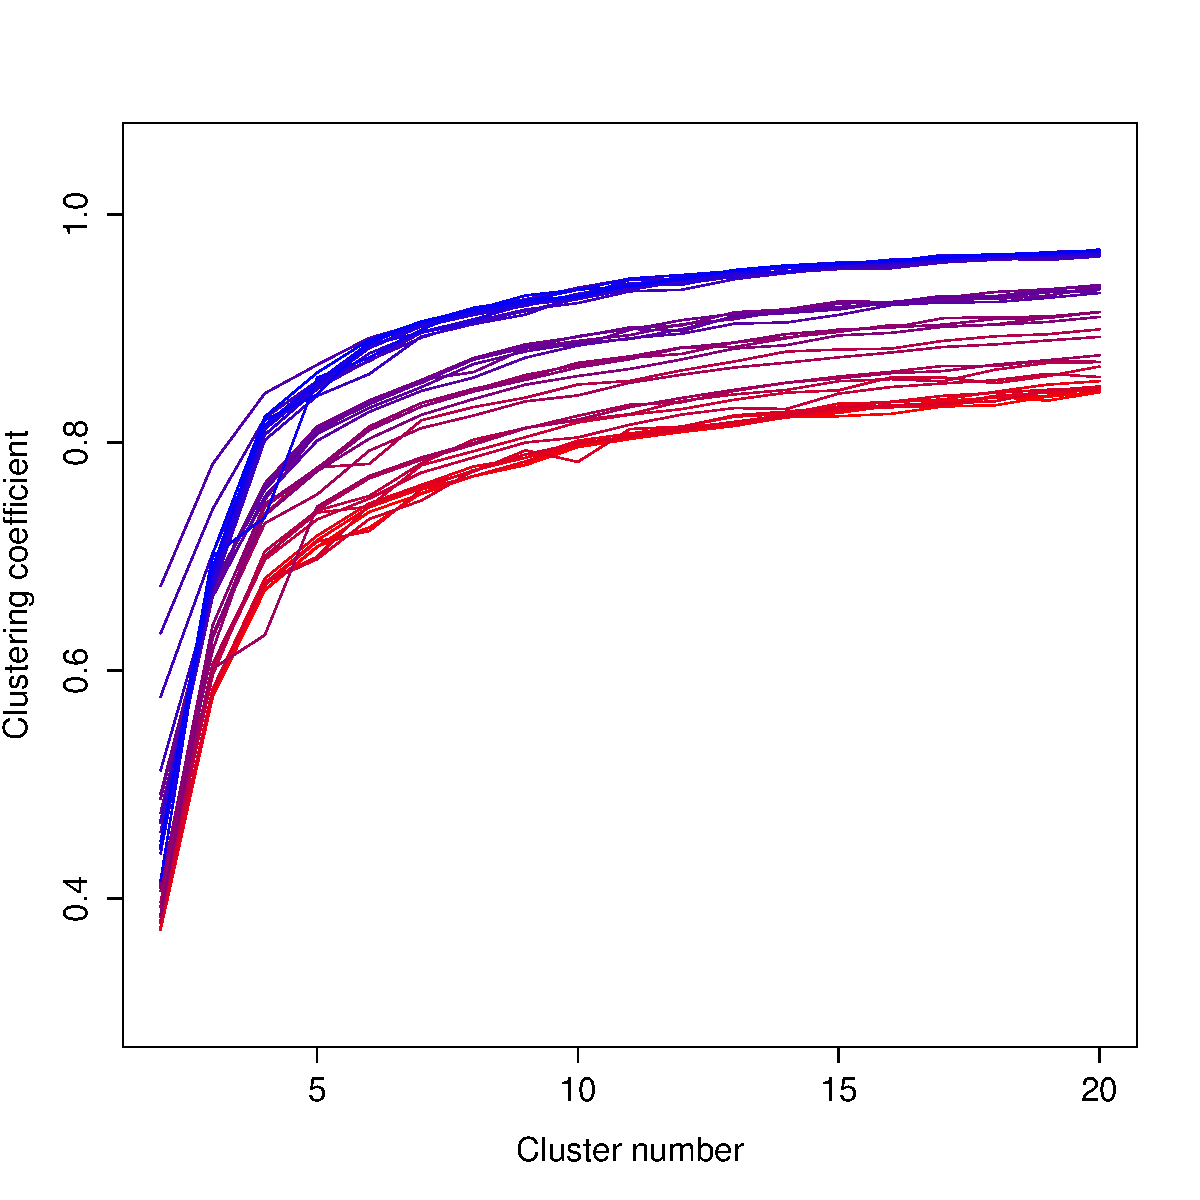
\includegraphics[scale=0.35]{/Users/Juste/Documents/ComplexSystems/CityBikes/Results/Clustering/clusterNumber}



}\hfill{}\subfloat[Plot of the value of the clustering coefficient for k=2 (red) and
k=3 (green), as a function of sampling step. We see the significative
loss of information around a step of 400 minutes, which should correspond
to the disapearance of pics in the curve, since they contribute significantly
to the quantity of information.]{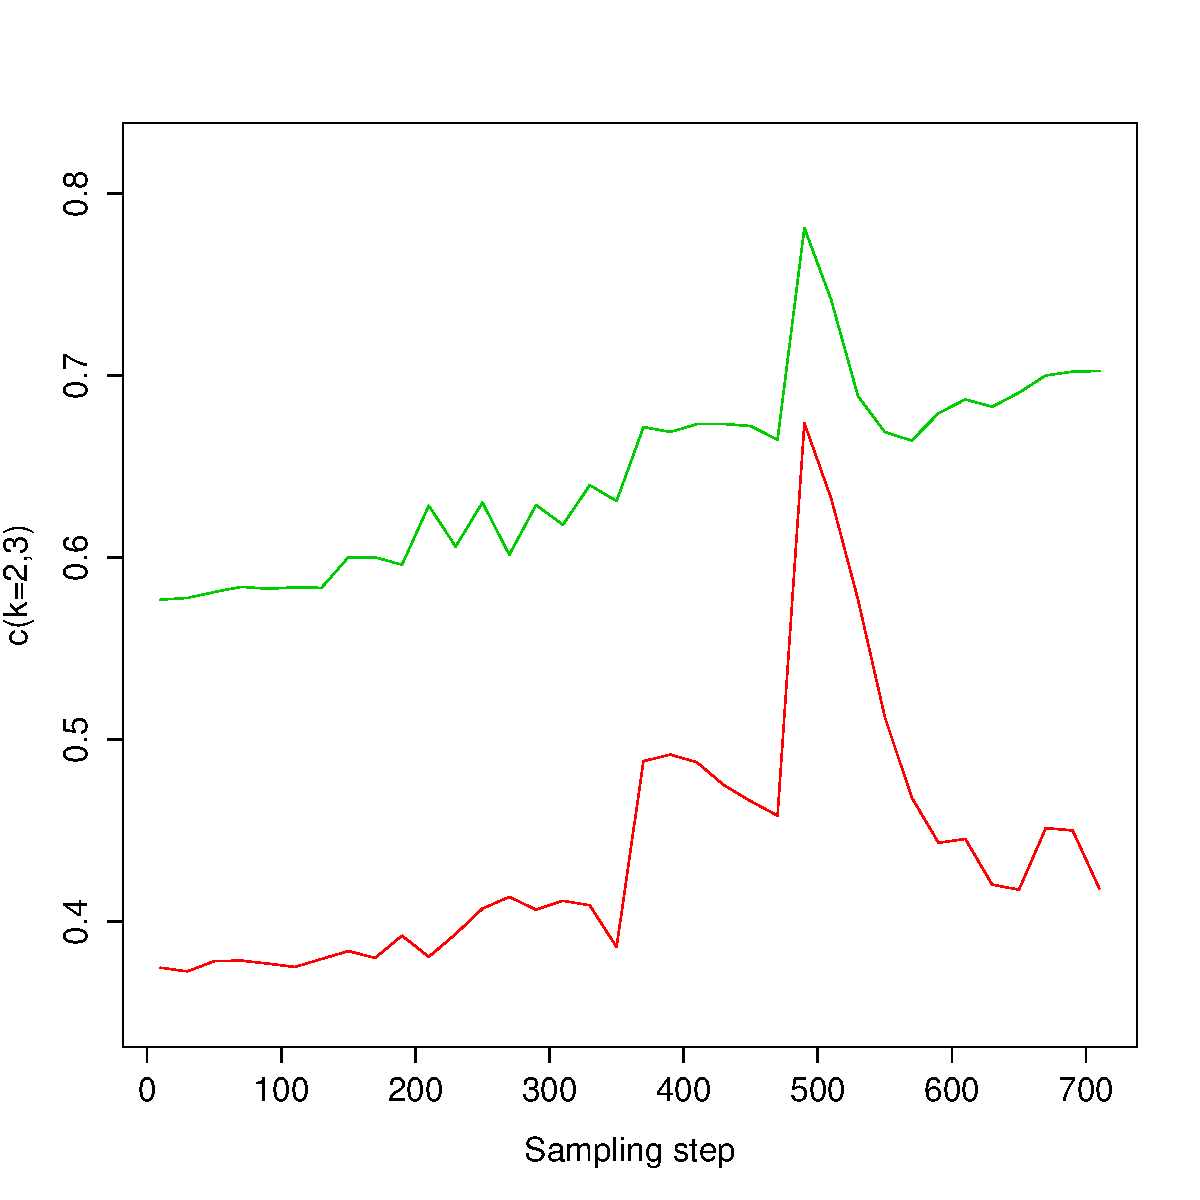
\includegraphics[scale=0.35]{/Users/Juste/Documents/ComplexSystems/CityBikes/Results/Clustering/infoLoss}

}\hfill{}

\caption{Influence of sampling interval on quantity of conserved information
in the clustering process.}


\end{figure}


We proceed then for each day to a k-means algorithm on the sampled
time-series (as described in \cite{warren2005clustering}), in order
to reduce more the dimension needed to represent a day. Intuitively,
that corresponds to a classification of stations according to their
``profile''. We take in practice 20 clusters, what allows to divide
by 100 the dimension. The final step is to cluster the representations
of the days for establishing a classification of days. With two clusters,
one expect to isolate weekdays from weekends, although kmeans can
lead to bad results if cardinal of clusters appear to be imbalanced.
In our case it worked quite well and we were able to reproduce that
distinction. However, a finer distinction (e. g. between rainy and
shiny days) was not possible and some work on a more specialized clustering
algorithm (kmeans is very general) would be needed to obtain more
precise results. Fig. 5 shows the comparison between real curves of
available bikes and predicted curves by the clustering algorithm.\bigskip{}


\begin{figure}
\hfill{}\subfloat[Curves of available bikes for all day of the week. Week days are superposed
and correspond to the curves with two pics. the green and the blue
curve are respectively saturday and sunday.]{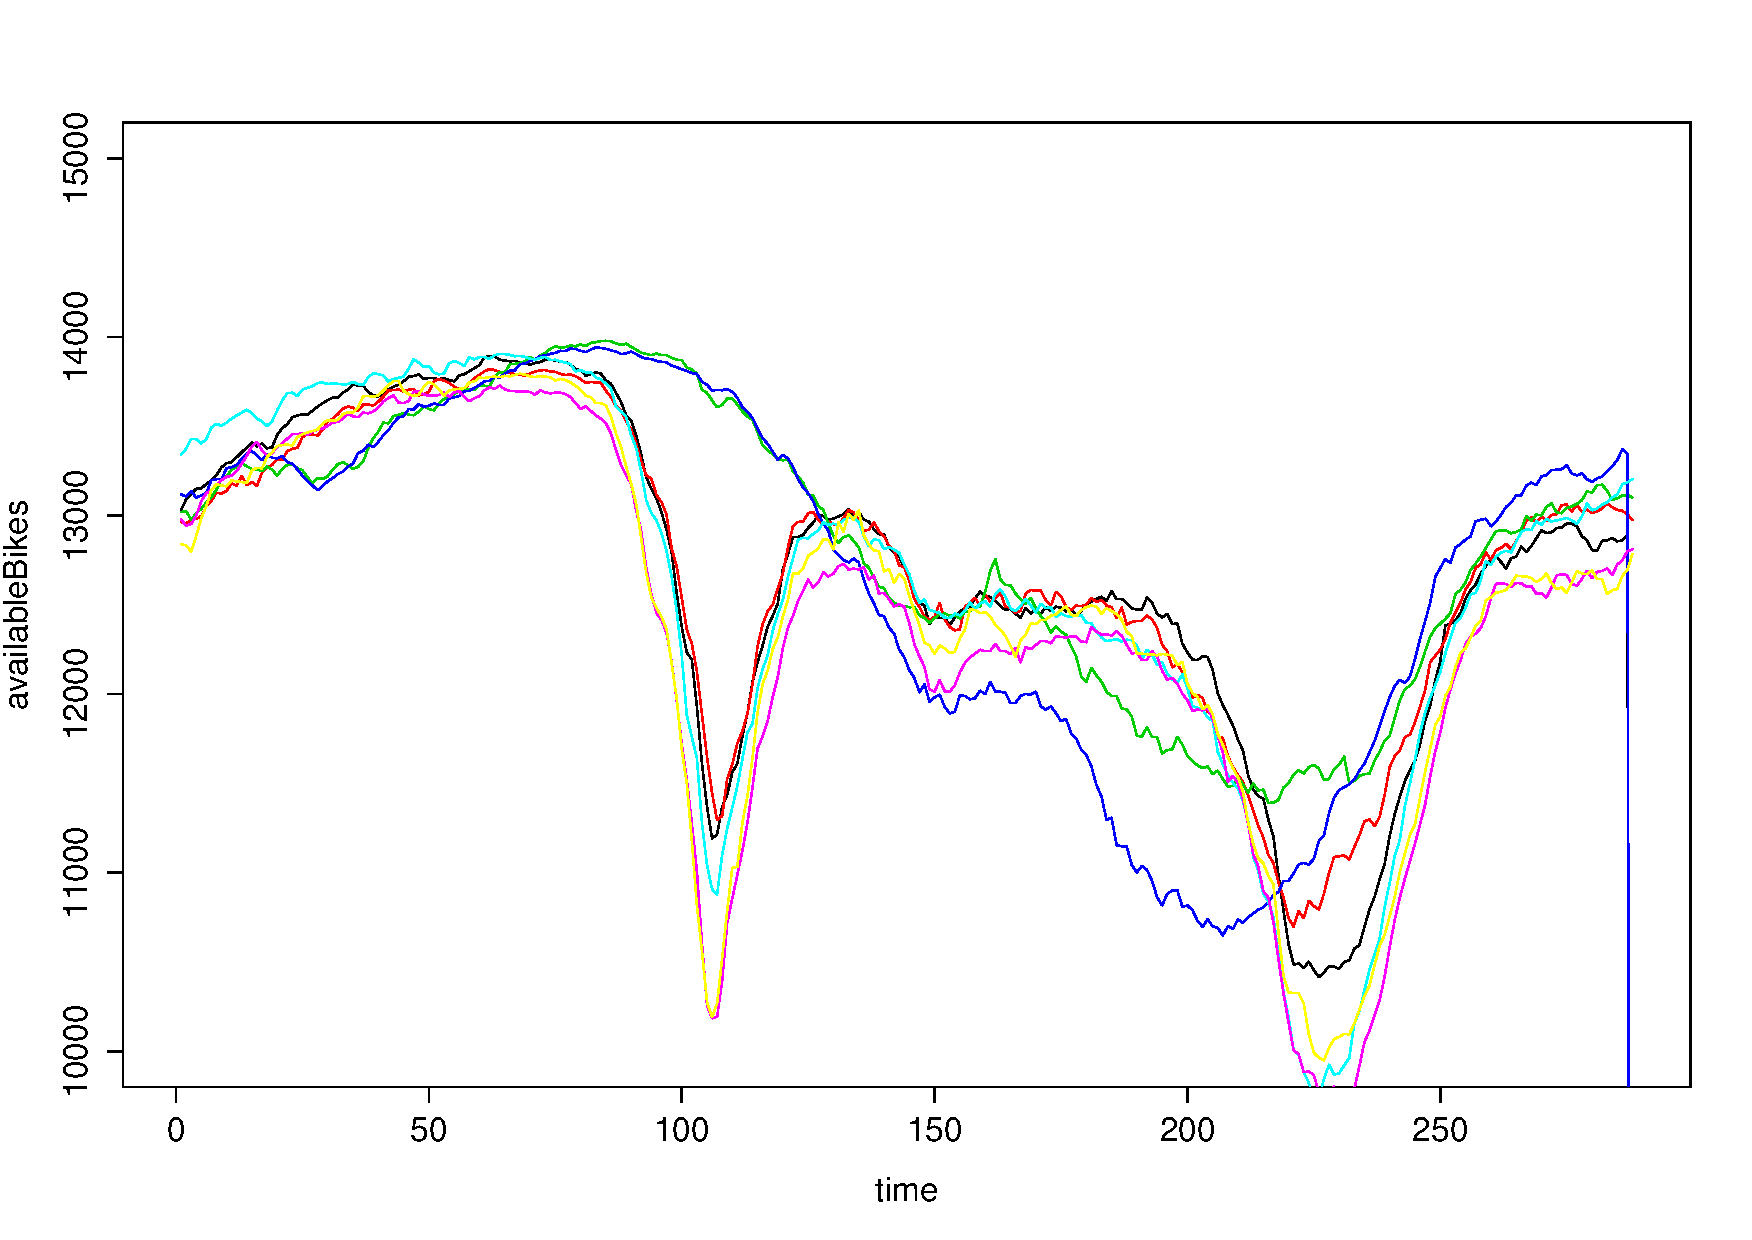
\includegraphics[scale=0.25]{/Users/Juste/Documents/ComplexSystems/CityBikes/Results/Clustering/week}

}\hfill{}\subfloat[Theoretical predicted curves for two clusters. As expected, we distinguish
week days (red curve) from weekend (blue curve), according to the
real curves.]{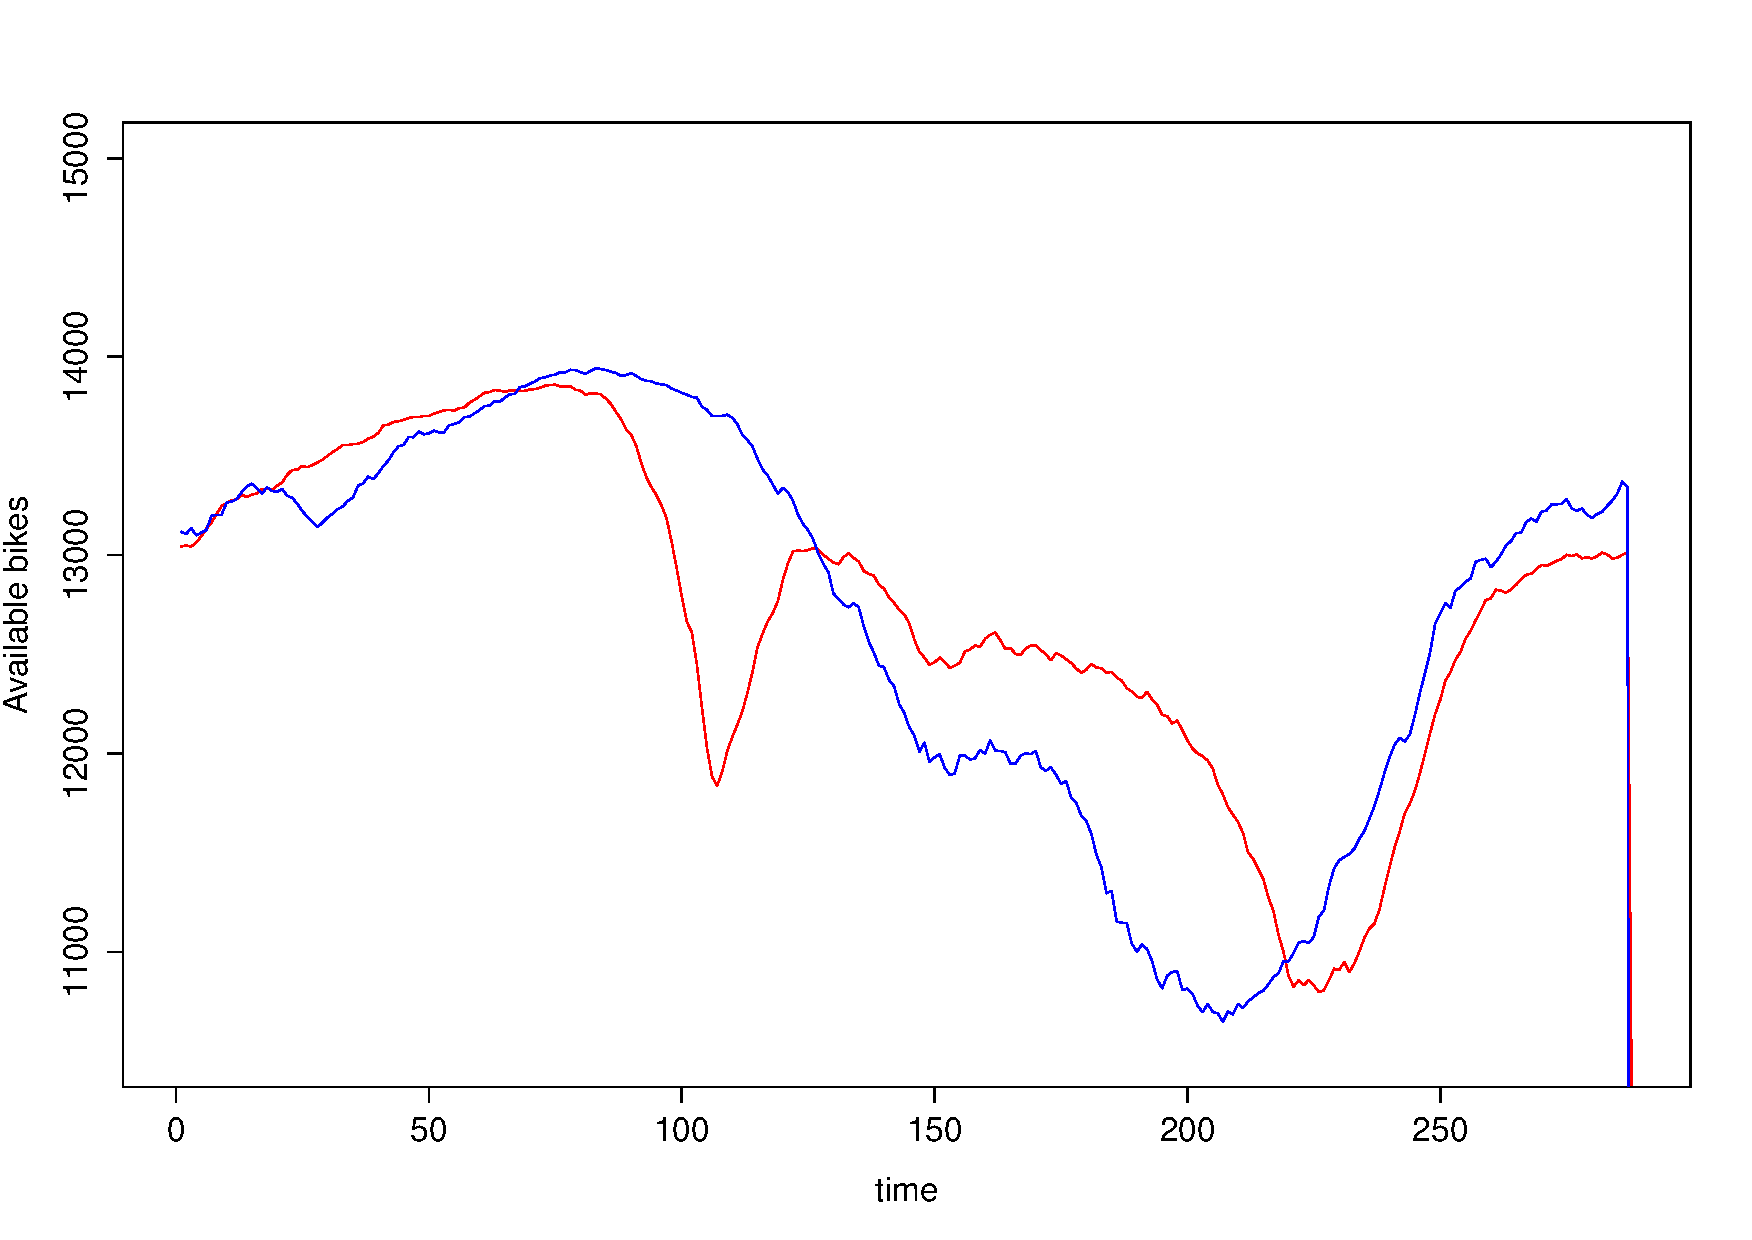
\includegraphics[scale=0.25]{/Users/Juste/Documents/ComplexSystems/CityBikes/Results/Clustering/curves}}\hfill{}

\caption{Results of clustering process for classification of days: distinction
between weekends and week days.}
\end{figure}



\subsection{Inference of origin/destination fields}

An other crucial point of the analysis is the estimation of real origin
and destinations of users of the system. If the original purpose is
in our case to obtain a parametrisation for an agent-based model as
we already explained, this problem has its own internal value. Indeed
a lot of research in economic geography and transportation geography
aims at evaluating real Origin/Destination fields in order to integrate
them into transportation/landuse models (see \cite{leurent2006modelisation}
for example).

\bigskip{}


Our statistical model for the inference of field is a non-parametric
estimation with Gaussian kernels (described in \cite{tsybakov2004introduction}).
Considering the real departures and arrivals in bike stations (that
are easily calculated by discrete differentiation of data), we count
each as a contribution to the global field at the current time step,
smoothed with Gaussian kernel (that appeared to be enough in practice).
At time $t$ ,with a parameter $\sigma$ fixing kernel sizes (each
kernel has the same size, further work could be done to test the influence
of multiple sizes, weighted by the maximum of the kernel distribution
for example) and a set of effective arrivals $(d_{i}(t))$ at the
corresponding coordinates $(\vec{x}_{i}(t))$, the spatial field of
destinations is estimated as, with $K$ normalisation factor,
\[
[D(t)](\vec{x})=\frac{1}{K}\sum_{i}d_{i}(t)\cdot exp(\frac{\left\Vert \vec{x}-\vec{x}_{i}\right\Vert }{2\sigma^{2}})
\]


We do the same for the origin field. Kernel estimations are done with
the ergonomic package \texttt{kernlab} (\cite{karatzoglou2004kernlab}).
These extrapolated fields are then discretised and used as parametrisation
for the agent-based models. We also use them to extrapolate bicycle
flows on a day. Fig. 6 shows an example of an obtained field.

\begin{figure}
\hfill{}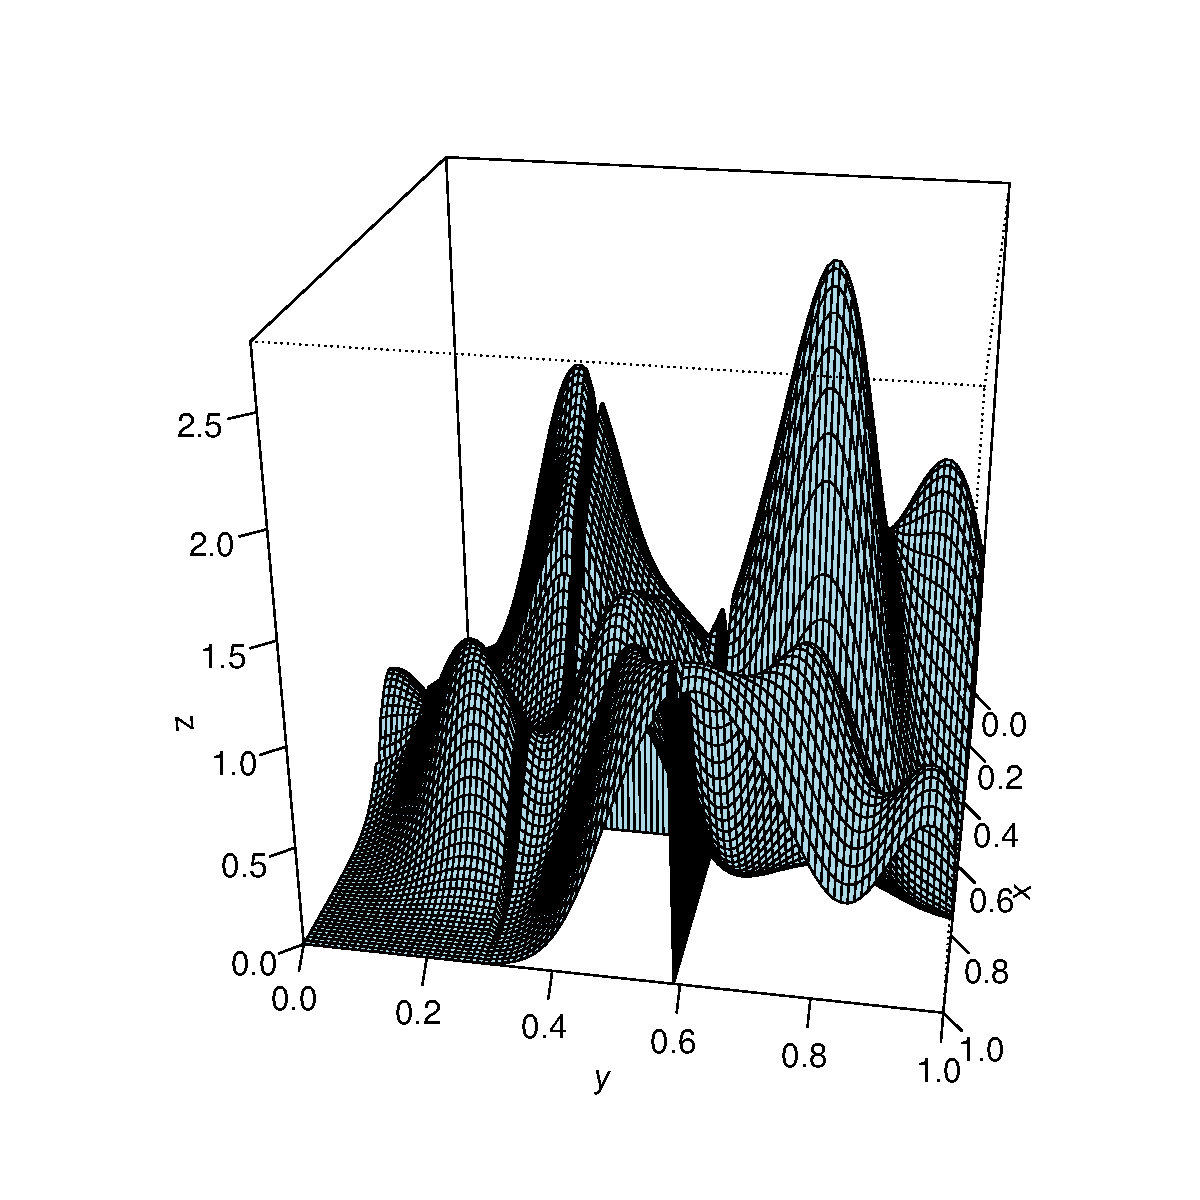
\includegraphics[scale=0.4]{/Users/Juste/Documents/ComplexSystems/CityBikes/Results/Kernel/example}\hfill{}\hfill{}\caption{Destination field obtained through Gaussian kernel estimation on a
square area.}


\end{figure}



\subsection{Mapping of bicycle flows}

One interesting application of the preceeding point is the extrapolation
and mapping of flows on a day. Especially, it allows to see if data
we have are enough to understand the mechanisms of the system, i.
e. infer reasonnably well possible travels, or if more would be needed.

\bigskip{}


Given mean time-series on a ``standard day'' (extracted through
clustering and mean of the larger cluster), we extract on all the
city the time-serie of effective departures and we calculate the origin
field. Then for each step of time, we draw randomly the expected number
of trips by the following process for each trip:
\begin{itemize}
\item Origin $\vec{o}$ is drawn from the origin probability field
\item Trip distance $r$ is drawn following a Gaussian law of mean 2km and
standard deviation 800m according to the distribution of travel distances
proposed in \cite{nair2013large}
\item We define the conditional destination field by $D_{r}(t)=K\cdot D(t)\cdot\mathbbm{1}_{\left\Vert \vec{o}-\vec{x}\right\Vert = r \pm \varepsilon}$,
where $\varepsilon$ is a tolerance parameter and $K$ a normalisation
factor and draw a random destination according to this field.
\item Following the shortest path between origin and destination in the
network, we increase by one the cumulated flow for each link.
\end{itemize}
\bigskip{}


That gives the map of the cumulated flows on a all day. Implementation
of GIS calculation and network paths was done in NetLogo (\cite{NetLogo})
in the frame of the agent-based modeling. Fig. 7 shows the obtained
map. We observe expected patterns in the center but irregularities
for some links, especially in south-east. However, we claim having
a good interpolation of the internal mechanisms of the system from
only partial data, answering partially to the question raised in 2.\bigskip{}


\begin{figure}
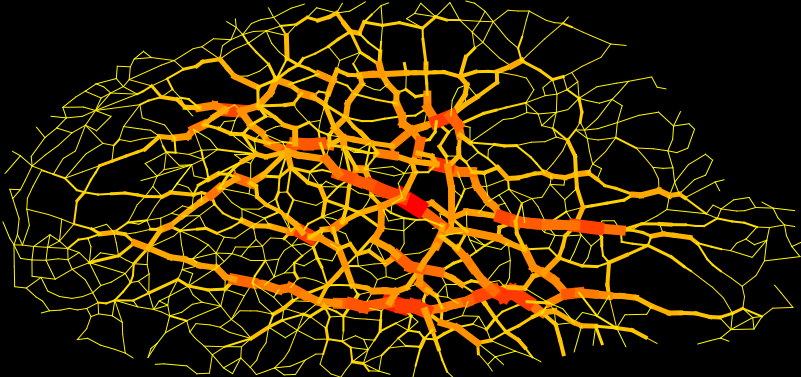
\includegraphics[scale=0.6]{/Users/Juste/Documents/ComplexSystems/CityBikes/Results/Mapping/BikingFlows}

\caption{Map of extrapolated cumulated flows on a day for Paris.}


\end{figure}



\section*{Conclusion}

We were able to proceed to statistical analysis of large data for
a better understanding of the working of a bike-sharing system. Although
results were sometimes quite limited, we showed that it was possible
to create knowledge from Open Data that were not aimed at that, what
is quite significant from an epistemological point of view. We argue
that it is a proof of the need of such data opening process, in all
fields, but also in a more extended way.\bigskip{}


Further development of that project could be a stronger assessment
and exploration of used methods, and also the insertion of methods
from other fields such as statistical medicine: considering redistribution
events as ``treatment'' on stations, and evaluating adverse events
as load-factor over a threshold for example, it would be able to consider
a district as a trial (treatment group: ay with redistribution, control
group without) and proceed to a meta-analysis on all district, in
order to quantify the effect of redistribution on the system. Such
transposition may however remain discutable and need to be considered
deeper.


\section*{Supplementary Material}

Source code of all statistical processing in R, data collection script,
and agent-based model in NetLogo (for the mapping part) in attached
zipfile.

\bibliographystyle{unsrt}
\bibliography{/Users/Juste/Documents/ComplexSystems/CityBikes/Biblio/bibtex,/Users/Juste/Documents/ComplexSystems/Biblio/BibTeX/global}

\end{document}
